\documentclass[a2paper]{article}

\usepackage{siunitx}
\usepackage{tikz}
\usepackage{amsmath}
\usepackage{geometry}
\usepackage{graphicx}

\newcommand*{\Scale}[2][4]{\scalebox{#1}{\ensuremath{#2}}}%

\geometry{a2paper,margin=0.5in}
\pagestyle{empty}

\begin{document}
\thispagestyle{empty}

% \begin{figure}[h!]
% \begin{tikzpicture}
% \node[anchor=south west,inner sep=0] at (0.2,-5.0) 
% {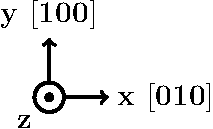
\includegraphics[width=0.30\textwidth]{arrows1}};
% \node[anchor=south west,inner sep=0] at (0.2,-0.3) 
% {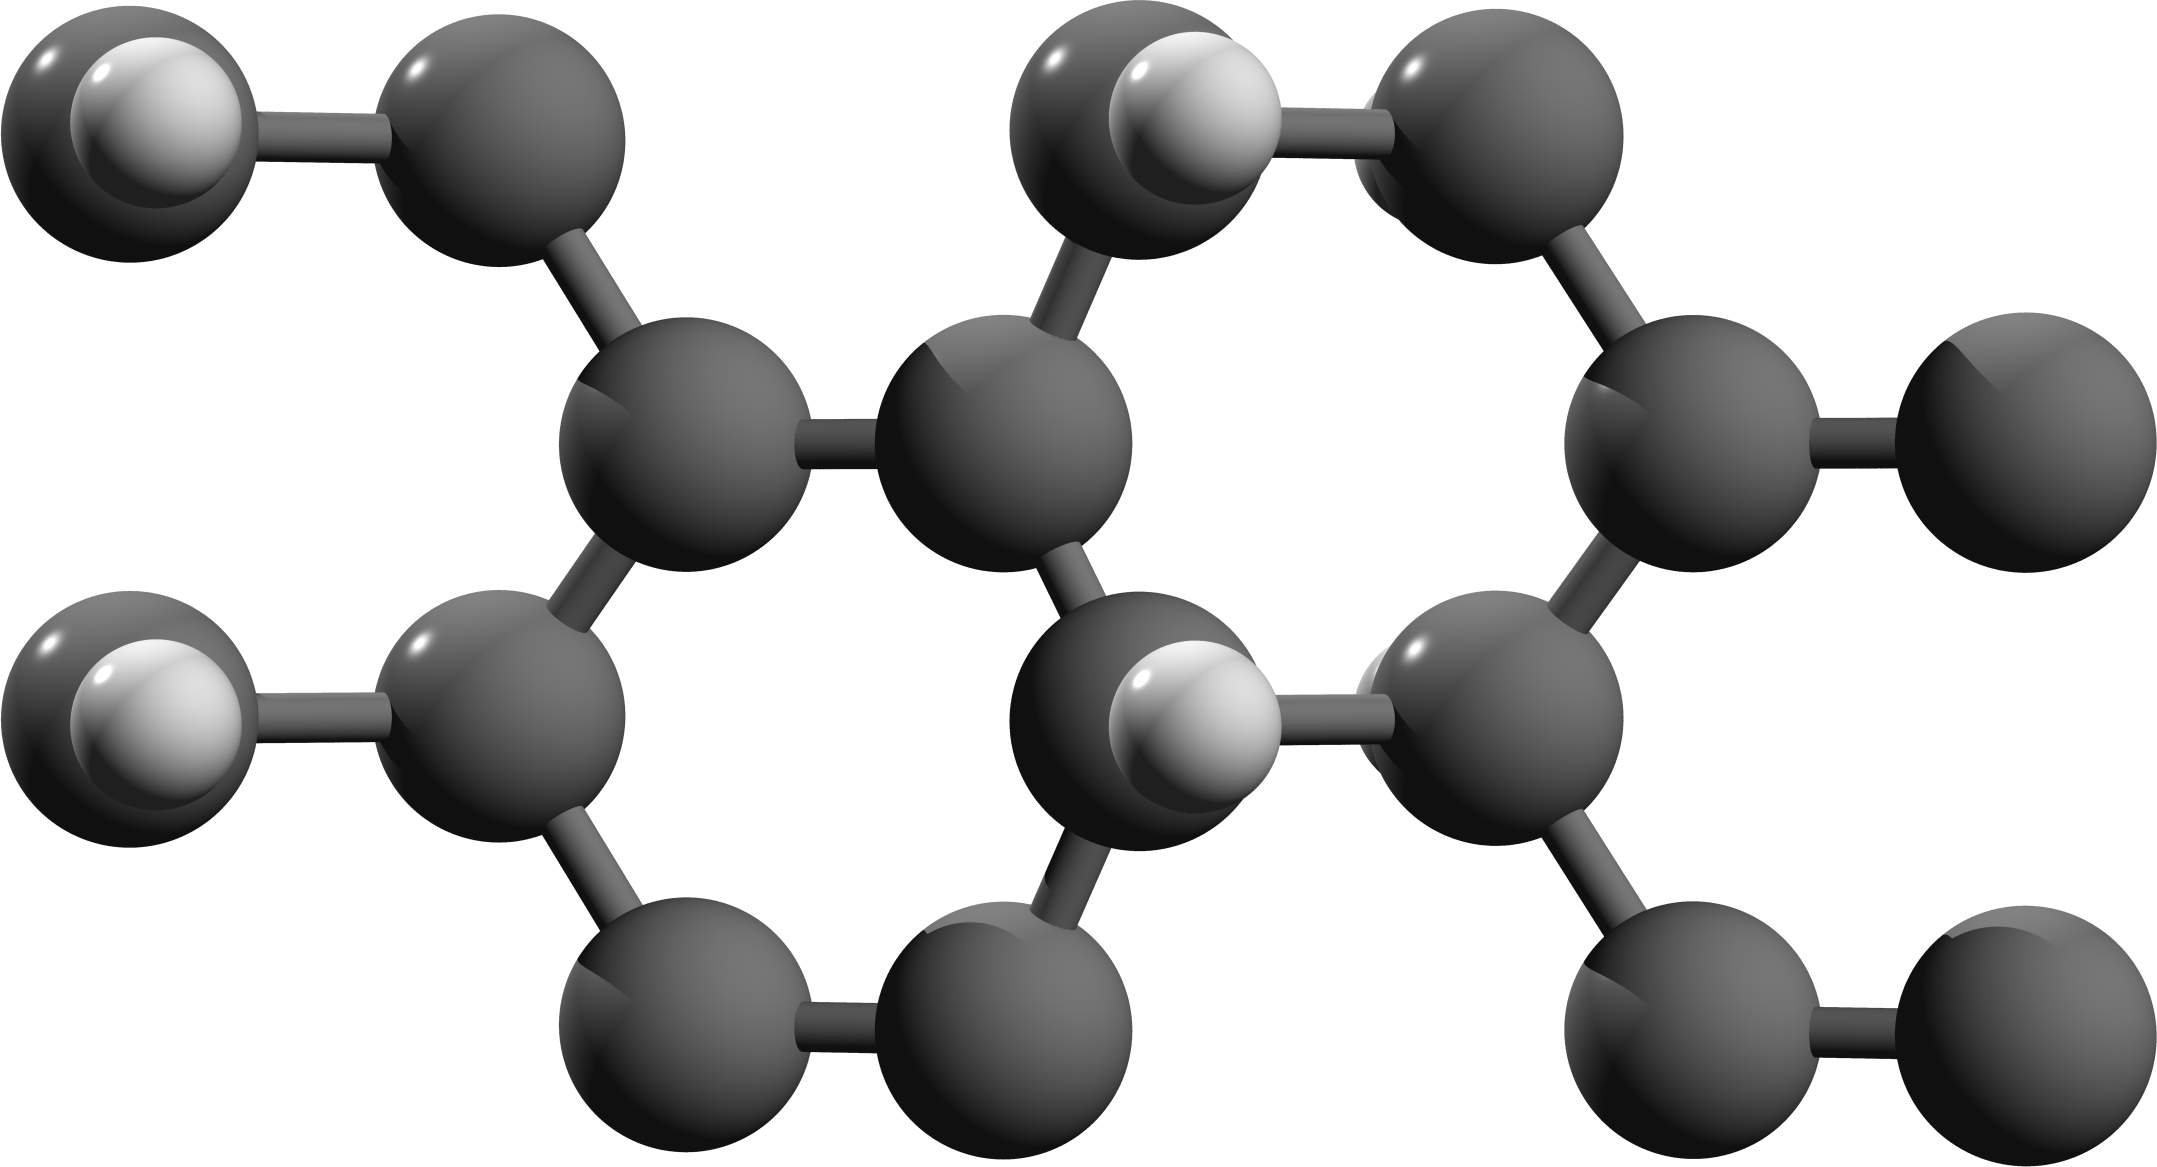
\includegraphics[width=\textwidth]{alt1}};
% \draw [line width=2.00mm, red ] (-0.30,05.00) -- (-0.30,10.80) node [right] {};
% \draw [line width=2.00mm, red ] (-0.30,10.70) -- (11.20,10.70) node [right] {};
% \draw [line width=2.00mm, red ] (11.15,10.76) -- (14.43,04.95) node [right] {};
% \draw [line width=2.00mm, red ] (14.37,05.00) -- (21.50,05.00) node [right] {};
% \draw [line width=2.00mm, red ] (21.40,05.10) -- (21.40,-0.60) node [right] {};
% \draw [line width=2.00mm, red ] (11.00,-0.50) -- (21.50,-0.50) node [right] {};
% \draw [line width=2.00mm, red ] (07.71,05.15) -- (11.08,-0.55) node [right] {};
% \draw [line width=2.00mm, red ] (-0.30,5.10) -- (07.78,5.10) node [right] {};
% \node[anchor=south west,inner sep=0] at (0.2,-34.0) 
% {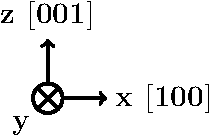
\includegraphics[width=0.30\textwidth]{arrows2}};
% \node[anchor=south west,inner sep=0] at (0.2,-24.6) 
% {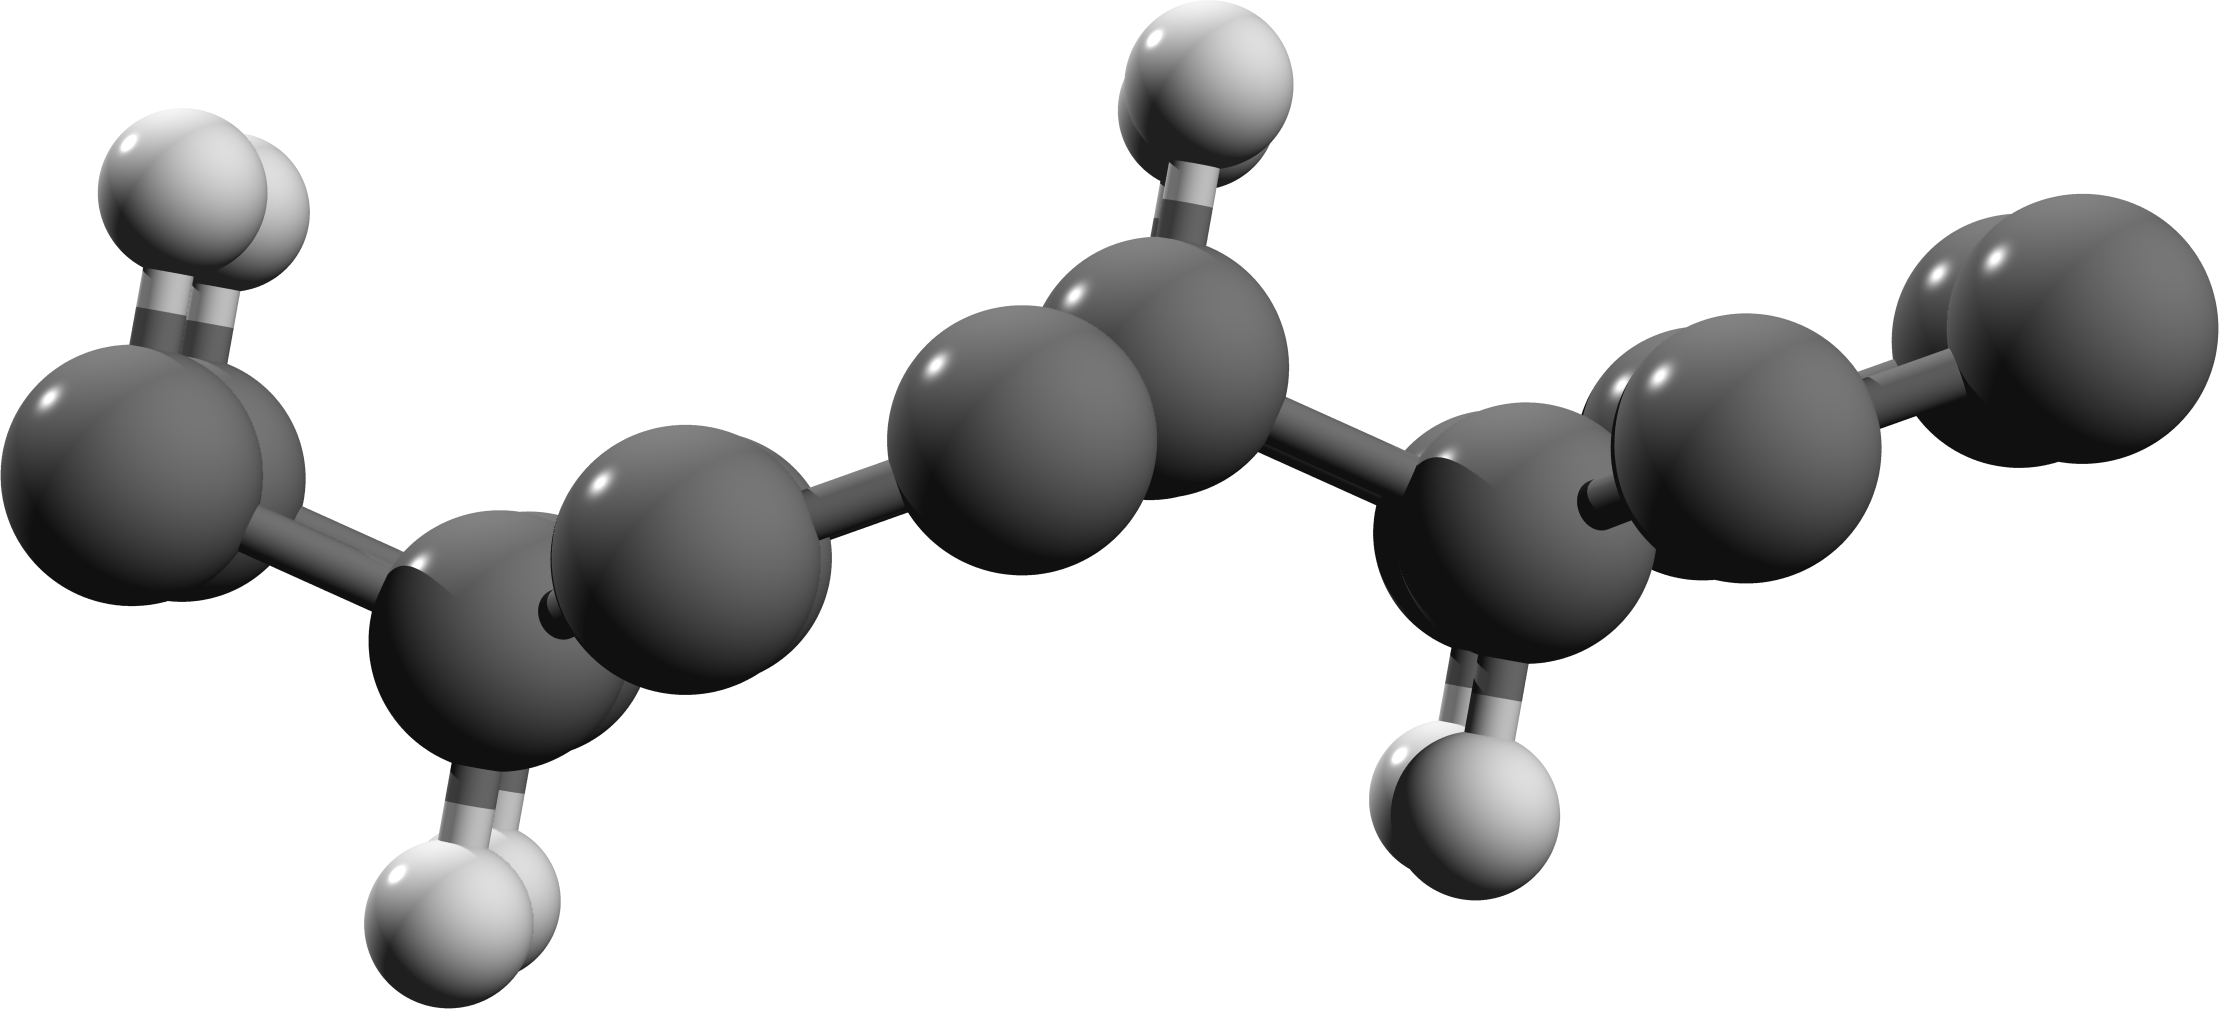
\includegraphics[width=\textwidth]{alt2}};
% \draw [line width=2.00mm, red ](-0.30,-25.20) -- (-0.30,-07.90) node [right]{};
% \draw [line width=2.00mm, red ](-0.30,-08.00) -- (21.40,-08.00) node [right]{};
% \draw [line width=2.00mm, red ](21.30,-25.20) -- (21.30,-07.90) node [right]{};
% \draw [line width=2.00mm, red ](-0.30,-25.10) -- (21.40,-25.10) node [right]{};
% \end{tikzpicture}
% \end{figure}

\begin{figure}[h!]
\begin{tikzpicture}
\node[anchor=south west,inner sep=0] at (0.2,-5.0) 
{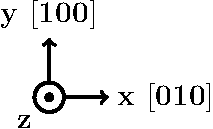
\includegraphics[width=0.30\textwidth]{arrows1}};
\node[anchor=south west,inner sep=0] at (0.2,-0.3) 
{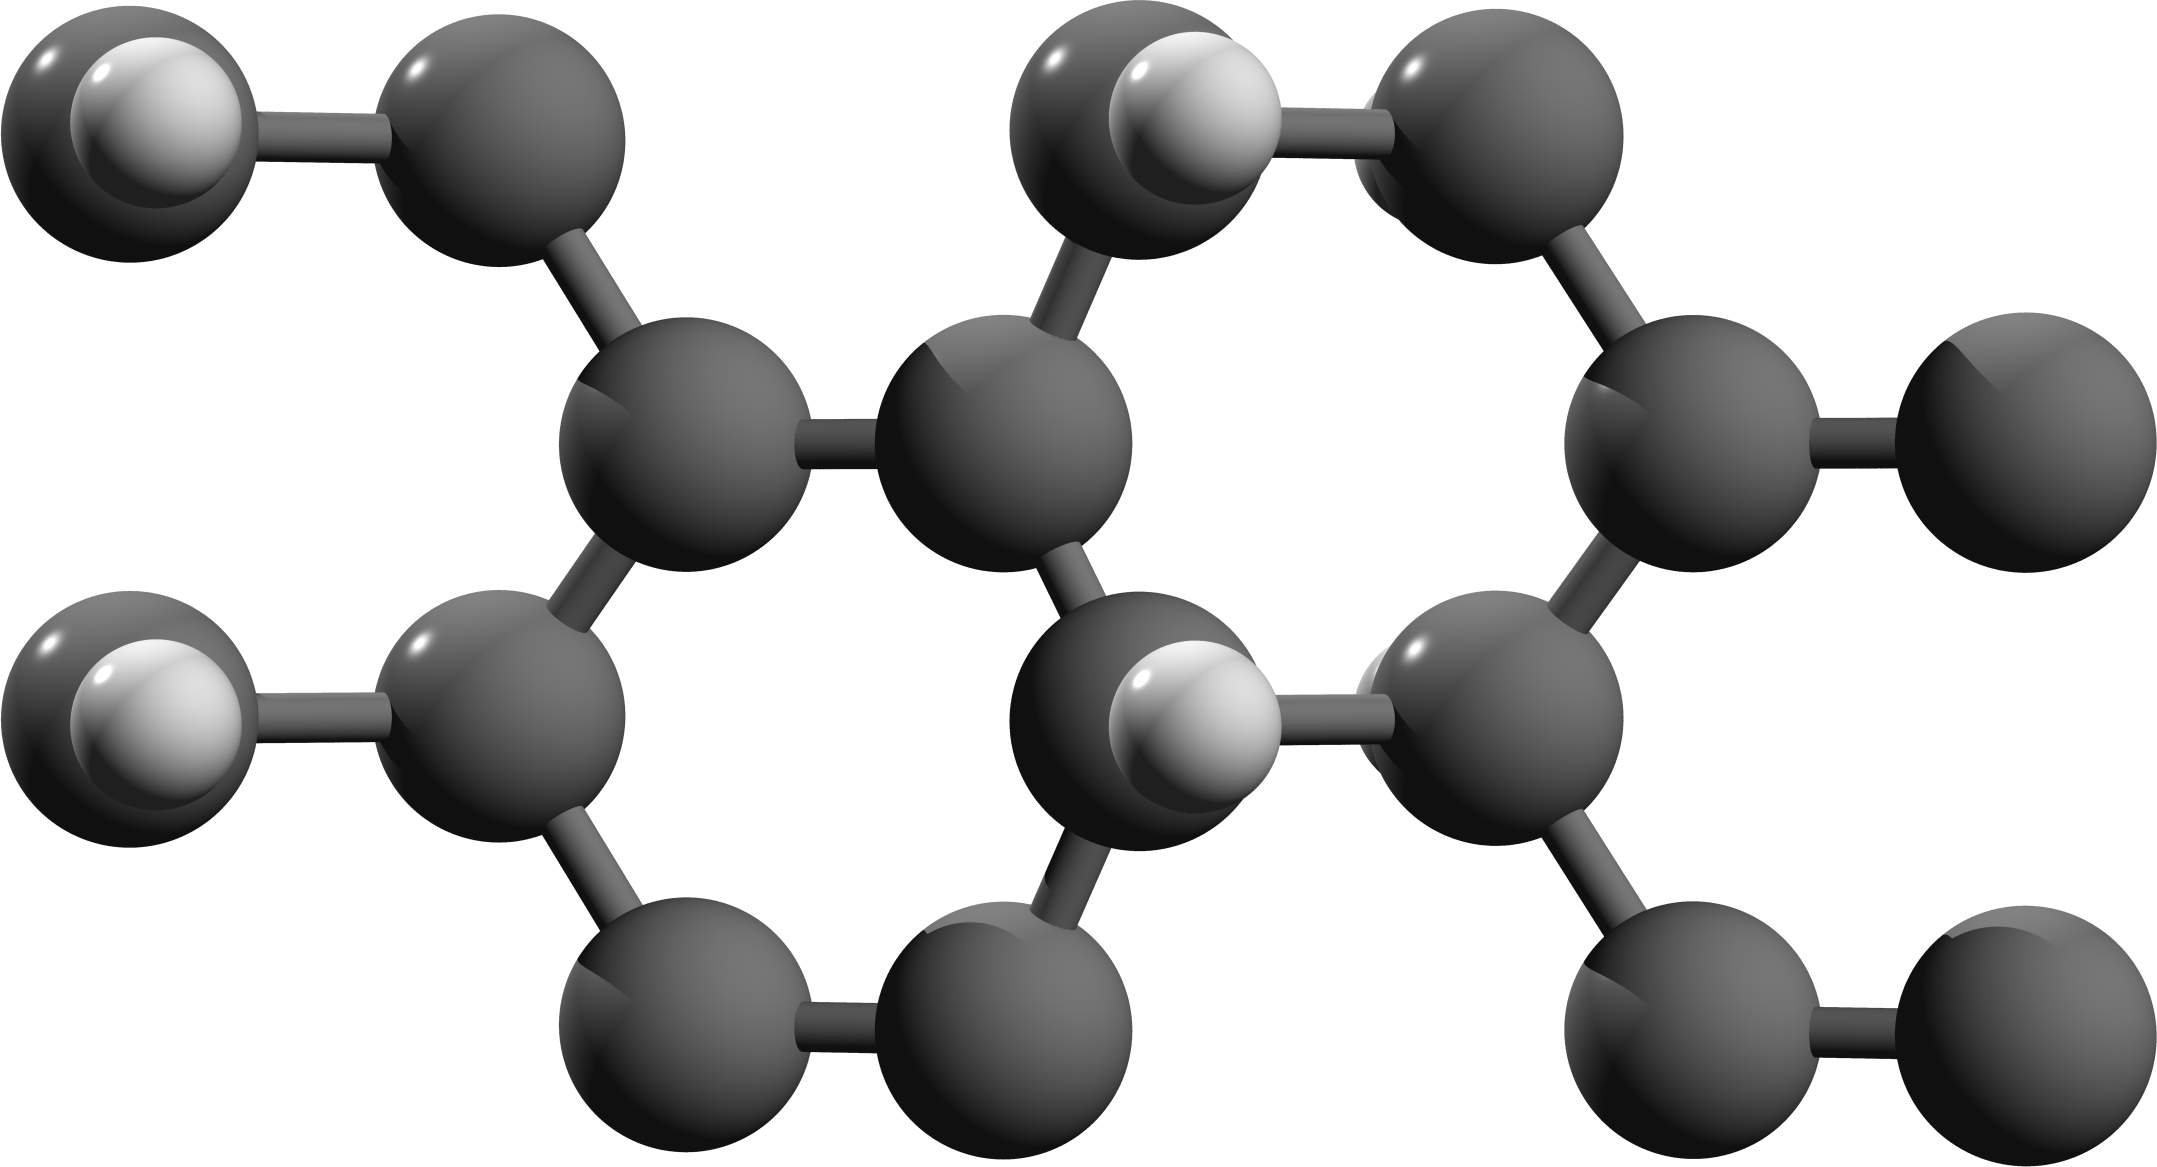
\includegraphics[width=\textwidth]{alt1}};
\draw [line width=2.00mm, red, -> ] (2.80,07.50) -- (2.80,19.00) node [right] {};
\draw [line width=2.00mm, red, -> ] (2.80,07.50) -- (22.00,07.50) node [right] {};
\draw [line width=2.00mm, red, dash pattern={on 10pt} ]
(22.00,07.50) -- (22.00,19.00) node [right] {};
\draw [line width=2.00mm, red, dash pattern={on 10pt} ]
(2.80,19.00) -- (22.00,19.00) node [right] {};
% 
\draw [] (-1.0,11.0) node [right] {\Scale[6]{\mathrm{C}_{1}}};
\draw [] ( 5.0,11.0) node [right] {\Scale[6]{\mathrm{C}_{2}}};
\draw [] (13.5,-1.0) node [right] {\Scale[6]{\mathrm{C}_{3}}};
\draw [] (19.5,-1.0) node [right] {\Scale[6]{\mathrm{C}_{4}}};
\draw [line width=2.00mm, <-] ( 3.5, 7.3) -- (5.0, 5.0) 
node [right] {\Scale[6]{\mathrm{H}_{1}}};
% 
\node[anchor=south west,inner sep=0] at (0.2,-34.0) 
{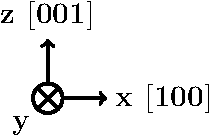
\includegraphics[width=0.30\textwidth]{arrows2}};
% 
\draw [] ( 1.0,-19.0) node [right] {\Scale[6]{\mathrm{C}_{1}}};
\draw [] ( 4.7,-20.0) node [right] {\Scale[6]{\mathrm{C}_{2}}};
\draw [] (13.0,-20.0) node [right] {\Scale[6]{\mathrm{C}_{3}}};
\draw [] (17.5,-18.5) node [right] {\Scale[6]{\mathrm{C}_{4}}};
\draw [] (-1.0,-10.0) node [right] {\Scale[6]{\mathrm{H}_{1}}};
\draw [] ( 4.0,-23.5) node [right] {\Scale[6]{\mathrm{H}_{2}}};
% 
\node[anchor=south west,inner sep=0] at (0.2,-24.6) 
{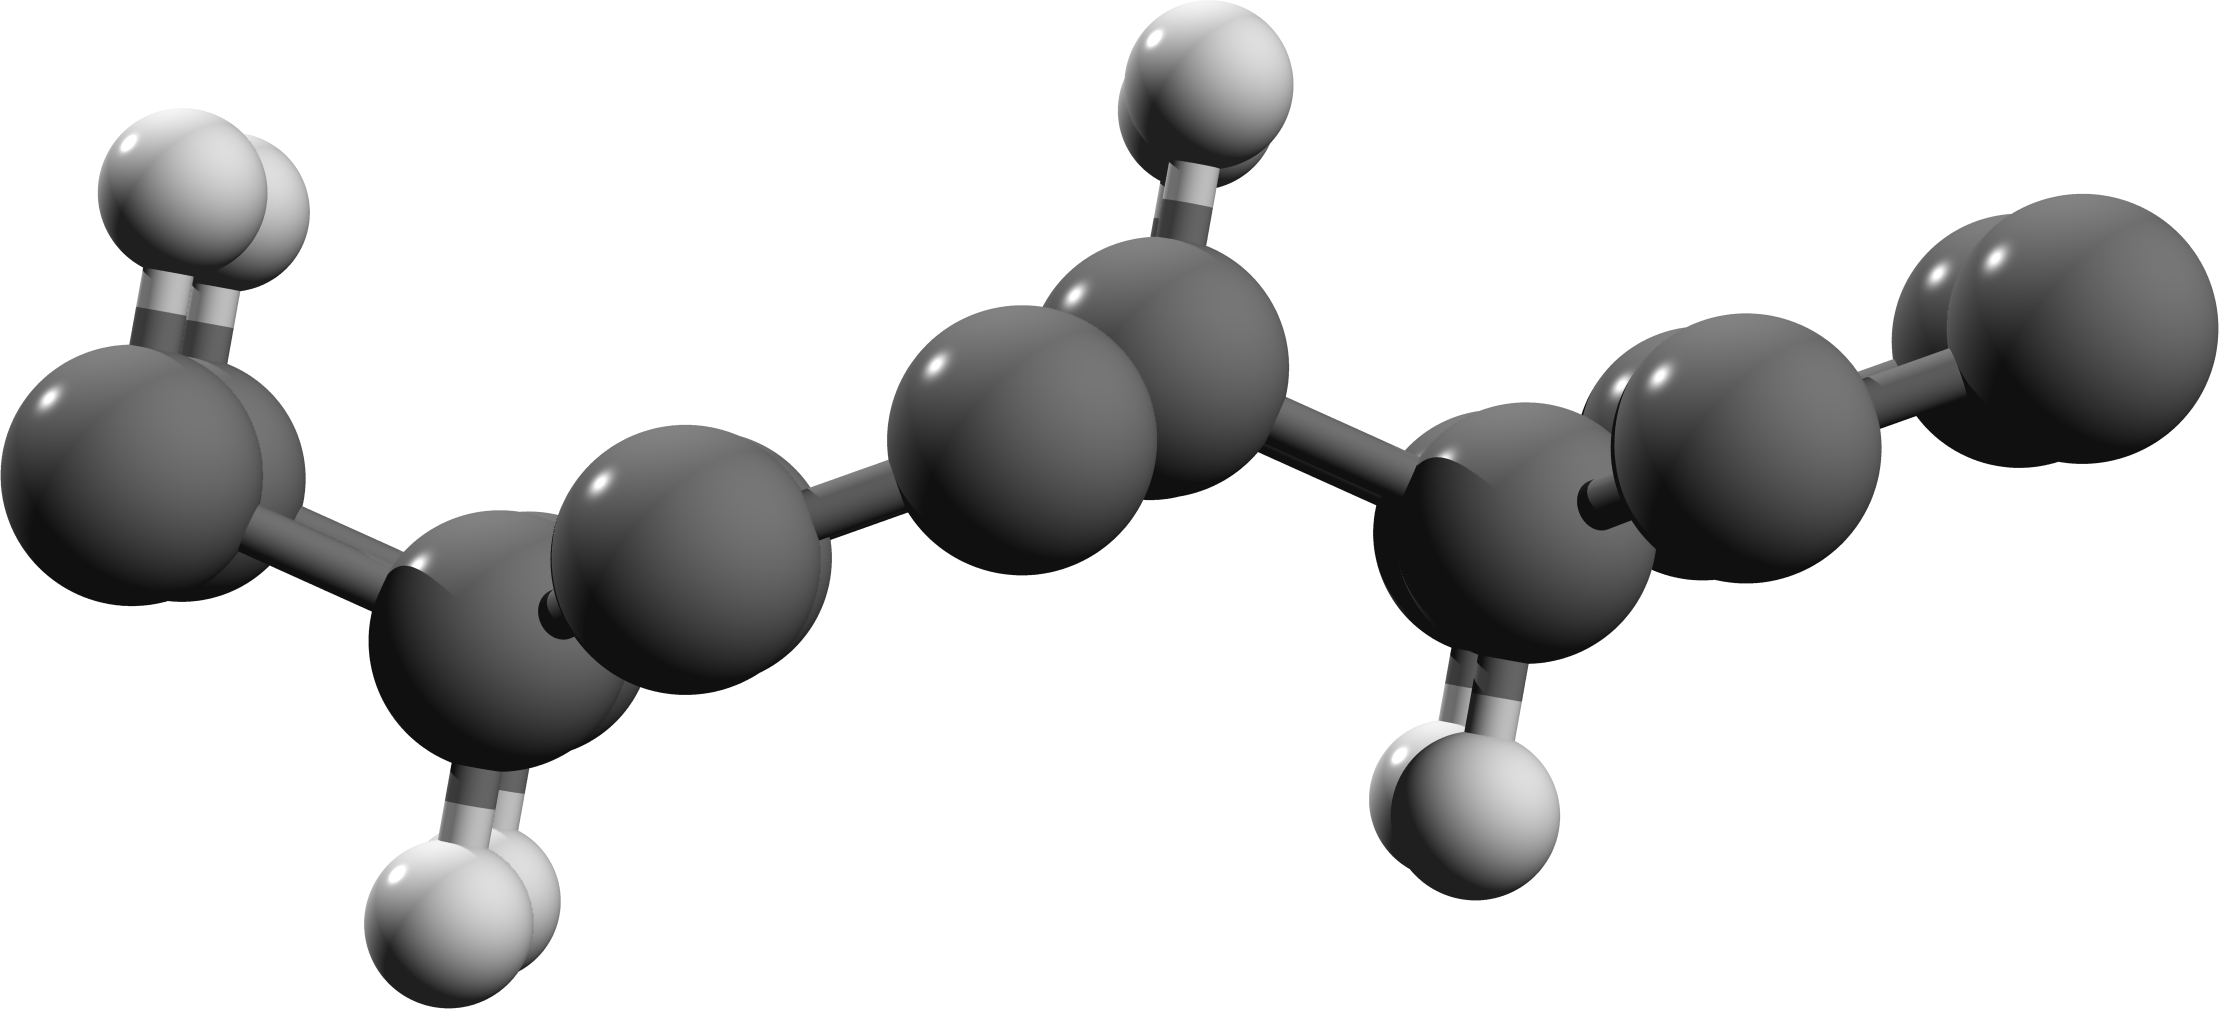
\includegraphics[width=\textwidth]{alt2}};
\end{tikzpicture}
\end{figure}

\end{document}
/Users/reinaldo/Desktop/structures/fig1.tex
